\documentclass{scrartcl}
\usepackage{tikz}

\setlength{\parindent}{0cm}

\title{CSC418 Assignment 1 Report}
\author{Philip Lee - 9999074932}
\begin{document}

\maketitle

\section{Introduction}


This program is an OpenGL implementation of a 9 degree of freedom (DOF) planar penguin. The 9 degrees of freedom are as follows: 
the penguin's limbs are able to rotate about its joints (6), the entire figure can be translated in the plane (2), 
and the penguin's beak is able translate in order to open and close (1). Each degree of freedom can be controlled via the spinners in the control bar.
The penguin can also be animated, in which case the magnitude of articulation for each limb is controlled via a sinusoid as a function of time.
Transformation hierarchies and a transformation stack were used to simplify the drawing of each limb in the correct location. 
The functionalities of the penguin can be separated into how it is animated, transformed, and drawn.

\section{Draw}


The body of the penguin is comprised of multiple irregular polygons. The head, body, arm, legs, and top beak were drawn by specifying vertices of each body part to OpenGL. 
OpenGL then connects the vertices but does not fill in the resulting polygon with a solid color. Parts such as the arm were relatively simple quadrilaterals, but 
other shapes such as the body had more vertices. These shapes were drawn within the coordinates of a unit square and scaled by transformation matrices in the transform function.\\

The shape of the feet was achieved by applying an additional shear transform to a square. The shear was achieved by rotating R degrees, scaling by constant alpha in X and Y, 
rotating -R degrees, and scaling by constant 1/Alpha in X and Y.\\

The joints of the penguin are circles. Since OpenGL is only capable of drawing straight lines, a circle was achieved by drawing a regular polygon with N=100 sides. This closely approximates a circle.\\

For shapes that are only drawn once such as the head or body, the colors are set when the shape's vertices are specified.\\

\section{Transform}


The transform function specifies the location, orientation, and size of each of the penguin's limb. When the screen is resized, the penguin is scaled such that it remains the same height, and translated so that it remains the same relative part of the window. Since the draw function assumes a unit square, the transform function is also responsible for scaling the length and width of each limb. The initial origin is considered to be the body. Each other limb is specified via a transformation tree from the center of the body. Specifically the transformation hierarchy is as follows:


\begin{figure}[!h]
 \centering
 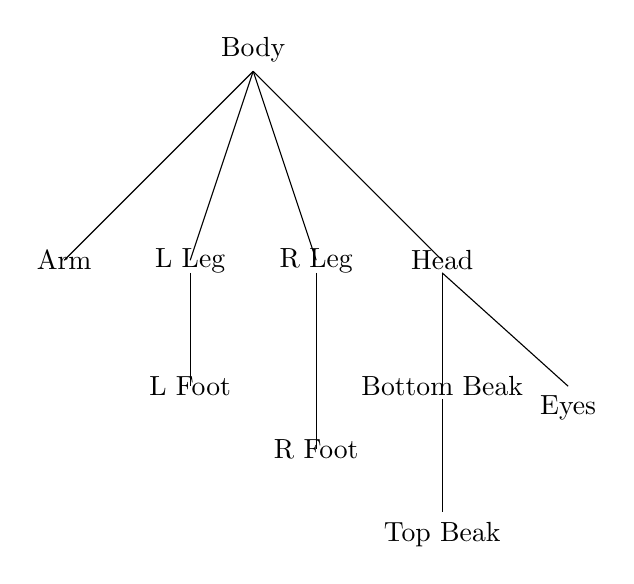
\begin{tikzpicture}[scale = 0.8]
  
    \draw (0,0) -- (-3,-3);
    \draw (0,0) -- (-1, -3);
    \draw (0,0) -- (1, -3);
    \draw (0,0)-- (3, -3);
    
    \node [above]at (0,0){Body};
    \node at (-3,-3){Arm};
    \node at (-1,-3){L Leg};
    \node at (1,-3){R Leg};
    \node at (3,-3){Head};    
    
    \draw (-1, -3.2) -- (-1, -5);
    \draw (1, -3.2) -- (1, -6);
    
    \node at (-1, -5){L Foot};
    \node at (1, -6){R Foot};
    
    \draw (3, -3.2) -- (3, -5);
    \node at (3, -5){Bottom Beak};
    
    \draw(3, -3.2) -- (5, -5);
    \node [below]at (5, -5){Eyes};
    
    \draw (3, -5.2) -- (3, -7);
    \node [below] at (3, -7){Top Beak};
    

 \end{tikzpicture}

 \caption{Transformation heirarchy.}
 
\end{figure}


For example, the location of the left foot is achieved by first translating the coordinate frame from the body to the left leg. The frame is then rotated to match the orientation of
the left leg, then it is translated to the left foot coordinate frame. Using such a hierarchy simplifies the matrix operations required to change coordinate frame because it is built
in steps that can be more easily observed and understood.\\

Rotation and translation of the degrees of freedom are accounted for in the transform hierarchy and ensure that a limb's pivot point is about the joint. To achieve rotation about
a point that is not the center of the shape, the shape is first translated such that the pivot point is lcoated at the origin. Then the rotation matrix is applied.\\

The values for the rotation and translation are updated in the animate function.		\\

\section{Animate}


When the animate option is enabled, the penguin's limbs move about their rotational or translational axes. The animate callback is executed. The maximum amplitude of rotation
for each limb is specified in the joint parameters. The animation values are updated every 50ms and follows a sinusoidal pattern. For the joints, a new rotation angle is calculated
every timestep, which is then used in the transform hierarchy to orient a limb. Some joints rotate faster than others, controlled by changing the frequency of the sinusoid. 
A similar method is applied to the beak, which translates up and down. The magnitude of translation is normalized to be between 0 and 1, with 1 being completely open and 0 being completely closed.

\end{document}